This chapter delves into the testing used for this project, including design and implementation specific details.

First, the purpose and method of testing are explored, followed by an overview of this method. The types of tests that have been undertaken in this project, and their design, are then illustrated. Finally, the testing environment is outlined, including details on the testing framework and how testing was performed.

\section{Purpose} {
\label{sec:testing_purpose}

	Software testing is performed to verify that a system successfully satisfies and implements the previously established user requirements. Another critical role of software testing is to locate and prevent defects created during the software development cycle. Ultimately, testing aims to provide information about the level of quality in a system, so developers can deliver a high quality product~\parencite{istqb2015testing}.

}

\section{Method} {
\label{sec:testing_method}

	This project has utilised the behavioural specifications, detailed in Section~\ref{sec:behavioural_specifications}, from behaviour-driven development (BDD), while maintaining a Rapid Application Development approach throughout development. This method of testing couples the advantages of RAD development, discussed in Section~\ref{sec:methodology} with the BDD approach outlined in Section~\ref{sec:behaviour_driven_development} below.

	\subsection{Behaviour-driven development} {
	\label{sec:behaviour_driven_development}

		Behaviour-driven development is an agile software development technique that focuses on obtaining a clear understanding of the desired software behaviour~\parencite{rice2014bdd}. It utilises an ubiquitous language, which is shared by software developers and management teams to extract and gather requirements, specifications and documentation~\parencite{bellware2015bdd, evans2004domain}. An important aspect of BDD is that the tests are highly granular, which enables programmers to determine points of failure more easily. Furthermore, BDD tests the system requirements, outputs the results in a natural human-readable format and provides living, up-to-date documentation of each system component.

	}

	\subsection{Behavioural specifications} {
	\label{sec:behavioural_specifications}

		BDD specifies behaviour through \emph{user stories}, which define the scope and acceptance criteria of the feature being tested~\parencite{north2007story}. A story template should contain all of the elements contained in the following template:

		\begin{verbatim}
			Title: a clear, explicit title describing the story
 
			Narrative:
			As a [role]
			I want [feature]
			So that [benefit]
			 
			Acceptance criteria: presented as scenarios
			 
			Scenario 1: Title

			Given [context]
			  And [some more context]
			When  [event]
			Then  [outcome]
			  And [another outcome]

	  		Scenario 2: ...
		\end{verbatim}

	}

}

\section{Testing types} {
\label{sec:testing_types}

	This project has undertaken the following types of testing:

	\begin{description}
		\item[Unit testing:] Validates the smallest components of a system, ensuring it handles known inputs and outputs correctly~\parencite{atlassian2015testing}.
			\begin{itemize}
				\item Unit tests should verify that the application works under expected, boundary, and negative cases.
			\end{itemize}
		% \item[System testing:] Verifies that a completely integrated system meets its requirements~\parencite{geraci1991ieee}.
		\item[Performance testing:] Determines the reliability, responsiveness, scalability, stability and throughput of a system under a particular workload~\parencite{microsoft2015performance}.
	\end{description}

	\todo{evaluate why I'm using these types}

	These tests have been performed 

}

\section{Test design} {
\label{sec:test_design}

	\todo{???}

	% http://blog.stevensanderson.com/2009/08/24/writing-great-unit-tests-best-and-worst-practises/

	% http://www.codeproject.com/Articles/5772/Advanced-Unit-Test-Part-V-Unit-Test-Patterns#Pass/Fail Patterns2

	% http://stackoverflow.com/questions/3840125/useful-design-patterns-for-unit-testing-tdd

	% http://programmers.stackexchange.com/questions/153410/what-are-the-design-principles-that-promote-testable-code-designing-testable-c
	
}

\section{Environment} {
\label{sec:testing_environment}

	The libraries used for the testing environment of this project have been outlined in Table~\ref{tab:testing_environment}.

	%!TEX root = ../report.tex

\begin{table}[H]
\caption[Testing environment]{The list of testing libraries used in the testing environment.}
\label{tab:testing_environment}
\begin{tabularx}{\textwidth}{@{}XX@{}}
	\toprule
	\textbf{Library} & \textbf{Description} \\
	\midrule
	Mocha & Testing framework \\
	Chai & Behaviour-driven development assertions \\
	Chai as promised & Promise assertions \\
	Sinon-chai & Spies, stubs and mocks \\
	Blanket & Code coverage \\
	Selenium & Automated browser testing \\
	\bottomrule
\end{tabularx}
\end{table}

}

\section{Testing framework} {
\label{sec:testing_framework}

	A testing framework is an execution environment for automated tests. They are responsible for defining a format to express expectations, test execution and reporting the results. Testing frameworks are application independent, easy to expand, maintain and are designed to help organise test suites to improve the efficiency of testing~\parencite{ghanakota2012testing}.

	\subsection{Choosing a testing framework} {
	\label{sec:choosing_a_testing_framework}

		There are many popular JavaScript testing frameworks available such as Intern, Jasmine, Mocha and QUnit which have been assessed below.

		\emph{Intern} supports functional testing, has a very simple setup and great user interface which has been highlighted in Figure~\ref{fig:intern}. It was difficult to locate a code coverage library that could be integrated with Intern, since it was released in \href{https://github.com/theintern}{2013} and has less overall support. When testing out this framework, it was extremely difficult to run custom configurations before test execution, since configurations were not particularly flexible. This also meant that it was challenging to run tests with the correct RequireJS dependencies, since Intern uses the Dojo AMD loader by default.

		%!TEX root = ../../report.tex

\begin{figure}[H]
	\centering
    \figureborder{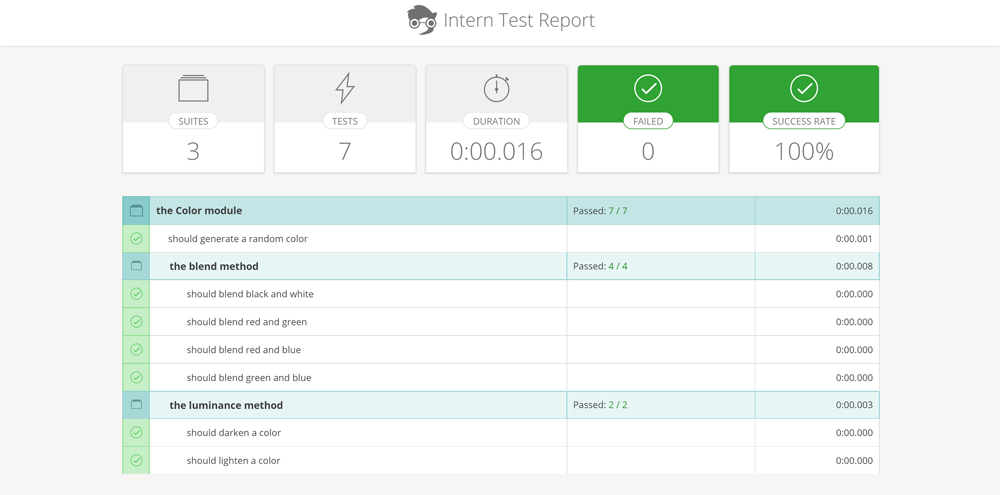
\includegraphics[width=\textwidth]{images/testing/intern}}
    \caption[Intern]{Intern user interface.}
    \label{fig:intern}
\end{figure}


		\emph{Jasmine} is often recommended and regarded as the most popular JS unit testing framework~\parencite{feldman2014testing}. It has a simple setup, built-in assertions, is well supported, can adapt to other assertion libraries and performs code coverage when used with Istanbul. Jasmine also has an elegant, descriptive syntax that adheres to the BDD paradigm. However, its asynchronous testing support could be improved greatly, which is problematic for this particular project because asynchronous loading is used extensively.

		\emph{Mocha} proved to have a very simple setup, is highly extensible, very flexible, has good reporting and a BDD syntax that resembles Jasmine. It allows the use of any assertion library, enabling users to choose their preferred BDD style and offers great asynchronous testing and promise support. Mocha can also be integrated easily with Blanket, a code coverage tool. One issue with Mocha is that it has an overly simple and plain user interface, sometimes making it difficult to determine which tests have passed or failed.

		\emph{QUnit} was immediately discarded since it does not support the BDD paradigm, and instead utilised TDD.

		Of these testing frameworks, \emph{Mocha} was chosen simply because of its fantastic asynchronous testing support and flexibility in choosing an assertion library and BDD style. Its user interface was transformed using customised CSS, which has been demonstrated in Figure~\ref{fig:mocha}, so the tests become more readable.

		\newcommand{\mochawidth}{0.496\textwidth}
\newcommand{\mochaheight}{4cm}
\begin{figure}[H]
	\centering
	\begin{subfigure}[b]{\mochawidth}
        \figureborder{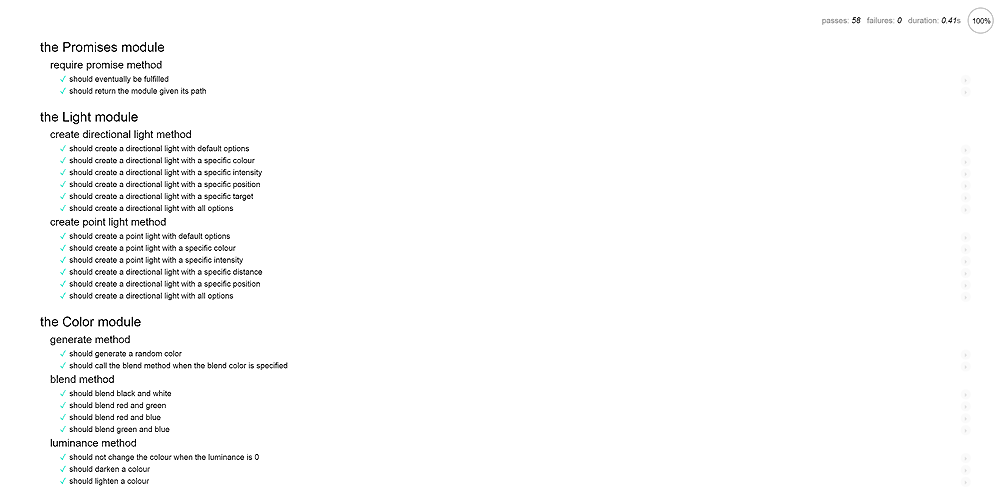
\includegraphics[width=\textwidth,height=\mochaheight]{images/testing/mocha_before}}
        \caption{Default Mocha interface.}
        \label{fig:mocha_before}
    \end{subfigure}
    \begin{subfigure}[b]{\mochawidth}
        \figureborder{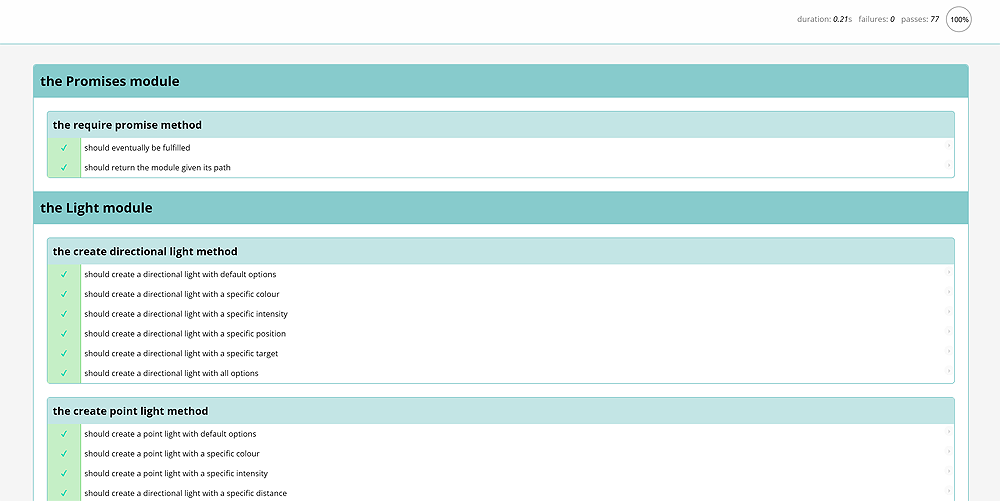
\includegraphics[width=\textwidth,height=\mochaheight]{images/testing/mocha_after}}
        \caption{Mocha interface after custom styling}
        \label{fig:mocha_after}
    \end{subfigure}
	\caption[Mocha]{Mocha styling}
	\label{fig:mocha}
\end{figure}


	}

% 	The intern (https://theintern.github.io/) test runner will be used along with the Chai assertion framework (http://chaijs.com/). This provides a familiar syntax as each test is written in AMD format. These allow for automated testing of both individual modules (unit tests) and simulating user clicks (functional tests) using selenium (http://www.seleniumhq.org/) with ChromeDriver (https://sites.google.com/a/chromium.org/chromedriver/).
% The intern also has support for running functional tests in a distributed manner across multiple machines on different operating systems via SauceLabs (https://saucelabs.com). This allows for further scalability in the future if the project is targeted to multiple systems.
% For mocking objects, SinonJS will be used (http://sinonjs.org/) alongside SquireJS (https://github.com/iammerrick/Squire.js/). Sinon-Chai will be used as well to integrate with the Chai assertions (https://github.com/domenic/sinon-chai).

}

\section{Unit testing} {

	Introduce setup.

	\subsection{Chai} {

	}

	\subsection{Chai as promised} {
	
	}

	\subsection{Sinon} {

	}

}

\section{Code coverage} {
	

}

\section{Performance testing} {

	Introduce setup.
	
	\section{Selenium} {

	}

}
